\documentclass{article}

\usepackage[dvips]{graphicx}
\usepackage{amsmath}

\renewcommand{\vec}[1]{\boldsymbol{#1}}

\begin{document}

\title{Mastering Singular Value Decomposition}

\author{Peter Mills}

\maketitle

\section{Introduction}

Every so often, maybe two or three times a decade, someone invents a 
mathematical technique or algorithm that changes the way we do things.
Maybe the method starts out in a small niche or field but eventually expands
to many other, completely unrelated disciplines and you cannot stop thinking
of new applications for it.
I'm talking about techniques like fast Fourier decomposition,
Monte Carlo integration, simulated annealing, Runge Kutta integration
and pseudo-random number generation.
I like to call such methods, ``power tools".
Singular value decomposition or ``SVD'' is one such method.

This introduction to assumes you have a good working knowledge of 
both matrix algebra and vector calculus.
We start with a short history of the method, then move on to the basic 
definition including a brief outline of numerical procedures.
This is then followed by a more intuitive derivation meant to demonstrate
the meaning of SVD.
The final section works out a complete program that uses SVD in a machine-learning
context.
Exercise are provided within the text.

\section{History}

The technique of singular value decomposition, or SVD for short, has a long
and somewhat surprising history.
It started out in the social sciences with intelligence testing.
Early intelligence researches noted that tests given to measure different
aspects of intelligence, such as verbal and spatial, were often closely
correlated.
Because of this, they hypothesized that there was a general measure of 
intelligence in common, which they called `g', now more commonly knwon
as ``I.Q.''
So they set about teasing out the different factors that made up intelligence
so as to pull out the most important one.

SVD is known under many different names.
In the early days, as the above passage implies, it was called, ``factor
analysis.''
Other terms include principal component (PC) decomposition and 
emprical orthogonal function (EOF) analysis.
All these are mathematically equivalent, although the way they are treated
in the literature is often quite different.

Today, the technique has spread through many branches of science in particular
psychology and socialogy, climate and atmospheric science, and astronomy.
It is also extremely useful in machine learning and in both descriptive and
predictive statistics.

\section{Technical introduction}

Singular value decomposition is a method of decomposing a matrix into three
other matrices as follows:
\begin{equation}
A = U S V^T
\label{SVD_def}
\end{equation}
where:
\begin{itemize}
\item $A$ is an $m \times n$ matrix, 
\item $U$ is an $m \times n$ orthogonal matrix,
\item $S$ is an $n \times n$ diagonal matrix
\item $V^T$ is an $n \times n$ orthogonal matrix.
\end{itemize}
The reason why the last matrix is transposed will become clear later on in the
exposition.
Also, the term, ``orthogonal'', will be defined (in case your algebra has become
a little rusty) and the reason why the two outside matrices have this
property made clear.

For the moment, we will assume that $m \ge n$.
What happens when this isn't true is quite interesting and is one of the keys,
in my opinion, to understanding SVD.

This is already becoming quite complicated so I will rewrite Equation 
(\ref{SVD_def}) using summation notation.
This is my go to method of proceeding whenever I am having trouble with a 
matrix equation.
In this case, while it doesn't make anything simpler, it does make everything
absolutely explicit:
\begin{equation}
a_{ij} = \sum_{k=1}^n u_{ik} s_k v_{jk}
\end{equation}
Note how we've collapsed the diagonal matrix, $S$, into a vector thus 
simplifying the expression into a single summation.
The variables, $\lbrace s_i \rbrace$, are called singular values and are normally arranged
from largest to smallest:
\begin{equation}
	s_{i+1} \le s_i
\end{equation}
The columns of $U$ are called left singular vectors while those of $V$ are
called right singular vectors.

We know that $U$ and $V$ are orthogonal, that is:
\begin{equation}
U^T U = V V^T = I
\label{ortho}
\end{equation}
Note that because $U$ is not square we cannot say that $U U^T=I$ so $U$ is 
only orthogonal in one direction.
Using the orthogonality property, (\ref{ortho}), we can rearrange (\ref{SVD_def}) into the following pair of eigenvalue
equations:
\begin{eqnarray}
A A^T U & = & U S^2 \label{U_eig} \\
A^T A V & = & V S^2 \label{V_eig}
\end{eqnarray}


\subsection{Numerical procedure}

Since $A^T A$ is the same size or smaller than $A A^T$, a typical procedure
is to plug (\ref{V_eig}) into an eigenvalue calculator to find $V$ and 
$S^2$ and then find $U$ by projecting $A$ onto $V$:
\begin{equation}
U = A V S^{-1}
\label{finding_U}
\end{equation}

Note that the method is completely symmetric; $U$ and $V$ change places
when $A$ is transposed:
\begin{equation}
A^T = V S U^T
\end{equation}
Thus, if $m < n$, we can transpose $A$, perform the decomposition, then
swap the roles of $U$ and $V$.
In this case, $U$ will be an $m \times m$ square matrix since there can 
at most $m$ non-zero singular values while $V$ will be an $m \times n$ matrix.

\subsection{Exercises}

\begin{enumerate}
	\item Use (\ref{U_eig}) and (\ref{V_eig}) to show that both $U$ and $V$ 
are orthogonal and that the eigenvalues, $\lbrace s_i^2 \rbrace$, are all positive.
\item Show that if $m < n$
there will be at most $m$ non-zero singular values.
\item Show that the eigenvalues in Equations (\ref{U_eig}) and 
(\ref{V_eig}) must be one and the same.
\end{enumerate}
\section{Understanding SVD}

\begin{figure}
	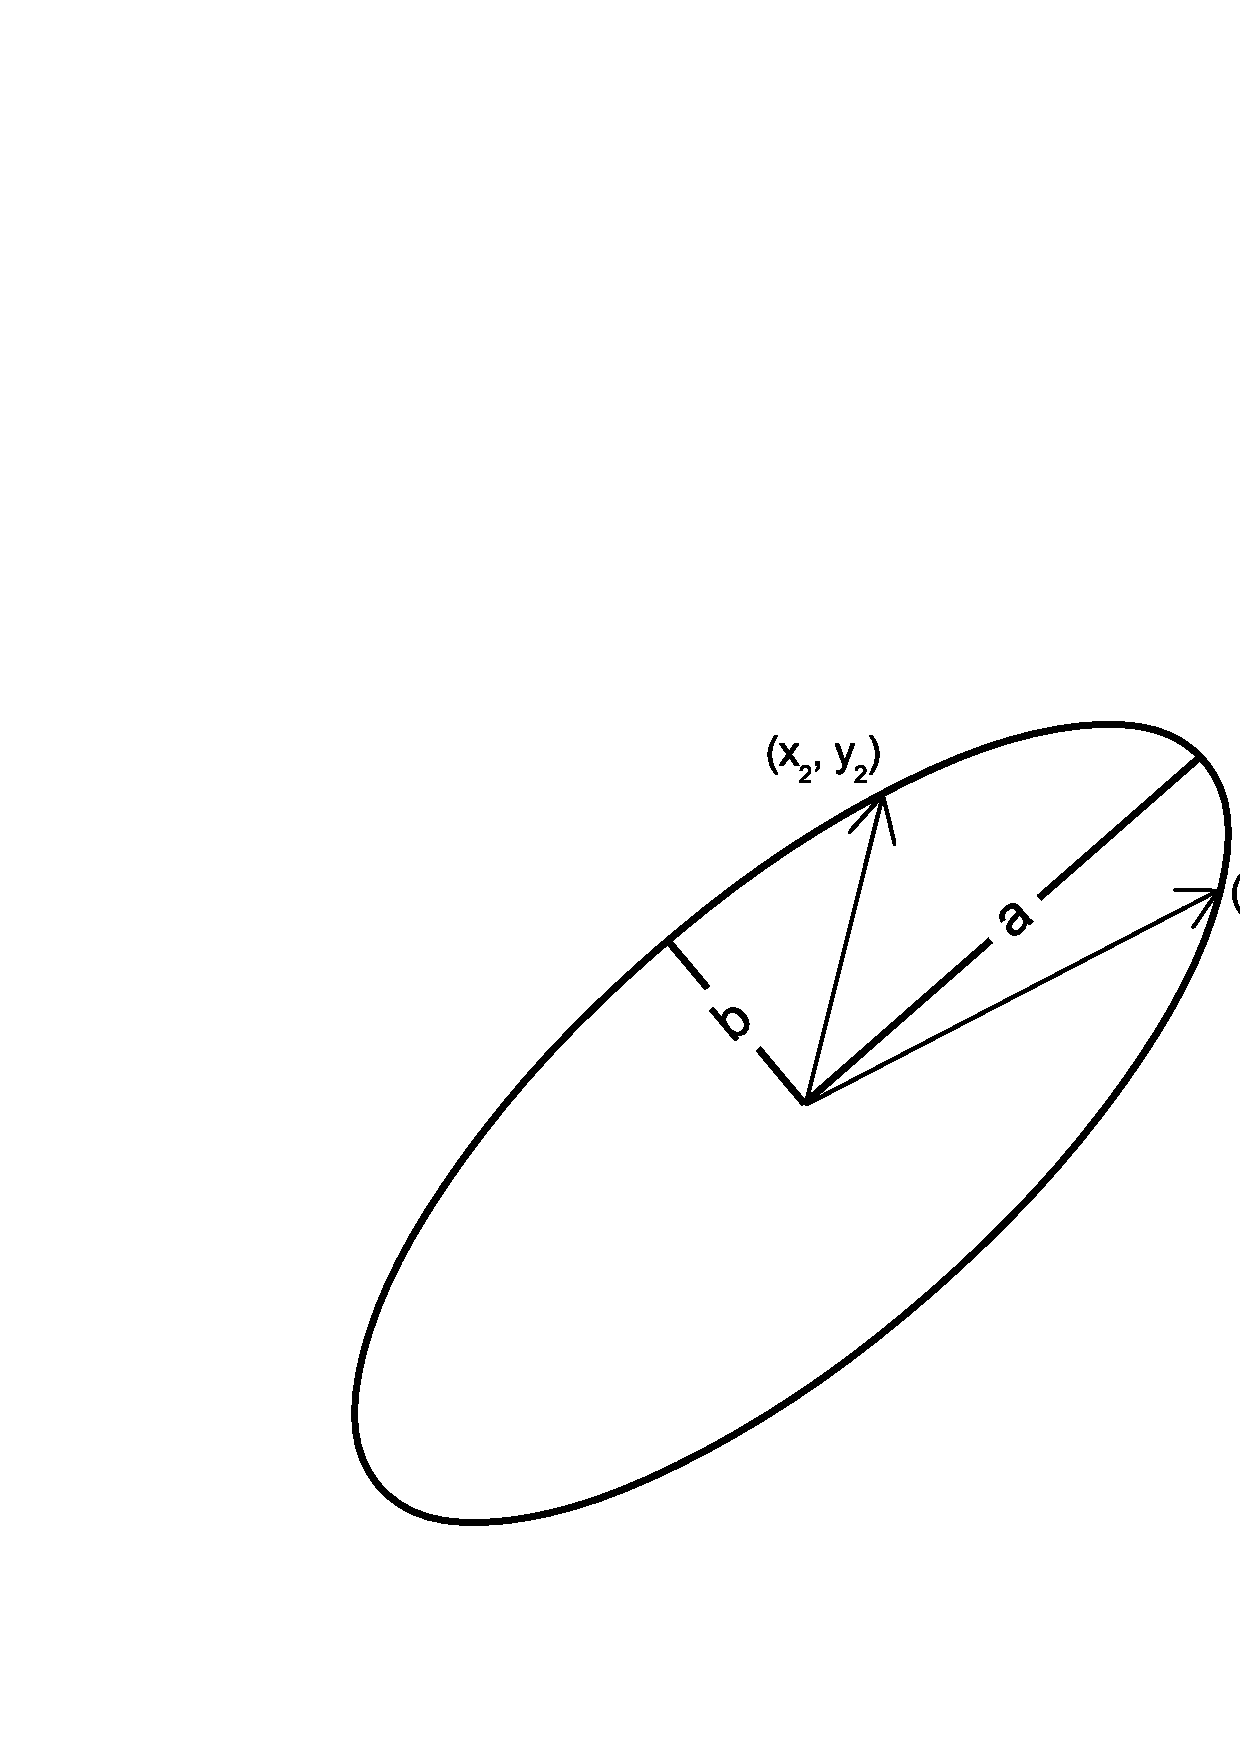
\includegraphics[width=0.9\textwidth]{svd_example}
	\caption{SVD in two dimensions.}
	\label{ellipse}
\end{figure}

Above is just the dry, technical jargon.
It doesn't give us an intuitive feel for what the method is doing.
So lets imagine the simplest example in two dimensions.
It generalizes very naturally to more.

Suppose we have two, two-dimensional vectors, $\vec x_1=(x_1,\,y_1)$, and 
$\vec x_2=(x_2,\,y_2)$.
We can fit an ellipse with major axis, $a$, and minor axis, $b$, to these two
vector as shown in Figure \ref{ellipse}.
But to make things easier on ourselves and save typing, we write out the 
equations using matrix algebra.

We can construct an ellipse of any size and orientation by stretching and
rotating a unit circle.
Let $\vec x^\prime=(x^\prime,\,y^\prime)$ be the transformed coordinates:
\begin{equation}
	\vec x^\prime = \vec x R M^{-1}
\end{equation}
where $R$ is a rotation matrix:
\begin{equation}
	R = \left [ \begin{array}{ll}
			\cos \theta & \sin \theta \\
			-\sin \theta & \cos \theta
	\end{array} \right ]
\end{equation}
and $M$ is a diagonal matrix containing the
major and minor axes:
\begin{equation}
	M = \left [ \begin{array}{rr}
			a & 0 \\
			0 & b
	\end{array} \right ]
\end{equation}
where $a$ and $b$ are the major and minor axes of the ellipse, respectively.

Lets write this out term-by-term, both for the general case:
\begin{equation}
	x_j^\prime = \frac{1}{m_j} \sum_i x_i r_{ij}
\end{equation}
where $m_i$ is the $i$th diagonal of the matrix, $M$;
and for the two-dimension case:
\begin{eqnarray}
	x^\prime & = & \frac{x \cos \theta - y \sin \theta}{a} \\
	y^\prime & = & \frac{x \sin \theta + y \cos \theta}{b}
\end{eqnarray}
Note that the rotation is clockwise, opposite the usual sense because we are
going from the untransformed to the transformed coordinate system rather than
the other way around. 
For the resulting ellipse, the angle will be in the usual, 
counter-clockwise sense.

The equation for a unit circle is as follows:
\begin{eqnarray}
	\vec x^\prime \cdot \vec x^\prime & = & 1 \\
	\left ( M^{-1} R^T \vec x \right ) \cdot \left ( \vec x R M^{-1} \right ) & = & 1
\end{eqnarray}
We wish to fit a set of $\vec x$'s, which we collect as the rows of a
matrix, $X$:
\begin{eqnarray}
	X & = & \left [
	\begin{array}{l}
		\vec x_1 \\
		\vec x_2 \\
		\vec x_3 \\
		...
\end{array} \right ] \\
& = & \left [ \begin{array}{ll}
x_1 & y_1 \\
x_2 & y_2 \end{array}
\right ]
\end{eqnarray}
The result is as follows:
\begin{equation}
M^{-1} R^T X^T X R M^{-1} = 1
\end{equation}
which is a rearrangement of equation (\ref{V_eig}).
If we regard $A$ as a collection of points, 
then the singular values are the axes of a least-squares fitted ellipsoid
while $V$ is its orientation.


\section{Applications}

The sum of the squares of the singular values should be equal to the total
variance in $A$.
Thus, the size of each tells you how much of the total 
variance is accounted for by each singular vector.
You can create a truncated SVD containing, for instance, only 99\% of the
variance:
\begin{equation}
a_{ij} \approx \sum_{k=1}^p u_{ik} s_k v_{jk}
\label{truncated_SVD}
\end{equation}
where $p<n$ is the number of singular values in the reduced system.
Typically, this will be fewer than the top ten ($p=10$) singular values.
It is in this facility of SVD to exclude the least significant components of
$A$ that its power lies.

\subsection{Solving matrix equations}

Some more rearrangement of (\ref{SVD_def}) shows that SVD can be used 
for solving systems of linear equations:
\begin{eqnarray}
A \vec x & = & \vec b \\
\vec x & = & V S^{-1} U^T \vec b
\label{matrix_solution}
\end{eqnarray}
or, in summation notation:
\begin{equation}
	x_i = \sum_j \frac{v_{ij}}{s_j} \sum_k u_{kj} b_k
\end{equation}
If this was all there was to it, there would be little to recommend SVD over
other matrix solvers such as QR decomposition or even Gaussian elimination.
In many cases, however, the matrix will be ill-conditioned, making the
solution unstable so that it blows up or produces floating point overflow. 
This will show up in the singular values: the smallest ones will be very close
to zero as measured relative to the largest.
To produce a stable solution, we just throw these components away as in
(\ref{truncated_SVD}) above.

This generalizes to non-square matrices. Since an $m \times n$ matrix, where
$m > n$, will have only $n$ singular values, in SVD this is equivalent to 
solving an $m \times m$ matrix using only $n$ singular values.
For non-square matrices, matrix inversion using SVD is equivalent to solving
the normal equation:
\begin{equation}
A^T A \vec x = A^T \vec b
\label{normal_equation}
\end{equation}
and produces the solution for $\vec x$ that is closest to the origin,
that is, of minimal length.
The normal equation is the solution to the following minimization problem:
\begin{equation}
\min_{\vec x} | A \vec x - \vec b|
\label{least_squares}
\end{equation}
Thus it is a generalized, least-squares fitting technique.

\subsection{Data reduction}

A typical machine learning problem might have several hundred or more
variables while many machine learning algorithms will break down if presented
with more than a few dozen.
This makes SVD indispensible in ML for variable reduction.
We have already seen in (\ref{truncated_SVD} how a SVD with a reduced number
of singular values can closely approximate a matrix.
This can be used for data compression by storing the truncated forms of
$U$, $S$, and $V$ in place of $A$ and for variable reduction by replacing
$A$ with $U$.
Any results will need to be transformed back to the original coordinate system
by multiplying with $S$ and $V$ in accordance with (\ref{finding_U}).

A full example including computer code will be worked out in the Example
section, below.

\subsection{Exercises}

\begin{enumerate}
	\item Show that Equation (\ref{matrix_solution}) is equivalent to 
Equation (\ref{normal_equation}).

\item Use Equation (\ref{least_squares}) to derive Equation (\ref{normal_equation}).

\end{enumerate}

\section{Example: variable reduction}

Suppose that the $m \times n$ matrix, $A$, stores a set of training data with 
each row a single training vector 
and that $n$, the dimension of each vector, is very large.
We want to feed $A$ to a clustering algorithm that outputs a fixed number of
cluster centers.
Because $n$ is large, however, the algorithms takes too long or is
unstable so we want to reduce the number of variables using SVD but in a way
that's transparent so it looks like we are still working in the un-trasformed
coordinates.

\subsection{Part 1: reading in the data}

To begin with, we will need to read in the data to fill up $A$.
I hope everyone understands C++:

\begin{verbatim}

#include <stdio.h>
#include <stdlib.h>

//subroutine header for performing singular value decomposition:
#include "svd.h"

//subroutine header for performing cluster analysis:
#include "cluster.h"

//maximum number of clusters:
#define MAX_CLUSTER 10

int main(int argc, char **argv) {
  char *infile;            //input file
  char *outfile;            //output file
  FILE *fs;                //file pointer
  double **a;            //matrix of training data/U
  int m;                //number of rows in matrix
  int n;                //number of columns in matrix
  int nsv;                //number of singular values

  if (argc!=4) {
    printf("syntax: cluster_svd nsv train centers\n");
    printf("  where:\n");
    printf("nsv      = number of singular values (0 = use untransformed data)\n");
    printf("infile   = ASCII input file containing training data\n");
    printf("output   = ASCII output file containing cluster centers\n");
    printf("\n");
    printf("file format:\n");
    printf("- one line header containing number of rows and number of columns\n");
    printf("- row major list of each matrix element\n");
    exit(1);
  }

  if (sscanf(argv[1], "%d", &nsv)!=1) {
    fprintf(stderr, "Error parsing first command line argument\n");
    exit(1);
  }
  infile=argv[2];
  outfile=argv[3];

  fs=fopen(infile, "r");
  if (fs==NULL) {
    fprintf(stderr, "Error opening input file, %s\n", infile);
    exit(1);
  }

  if (fscanf(fs, "%d %d", &m, &n)!=2) {
    fprintf(stderr, "Format error in input file: %s line 0", infile);
    exit(1);
  }
  if (nsv>n) {
    fprintf(stderr, "Command line parameter nsv=%d out of range\n", nsv);
    exit(1);
  }

  a=new double *[m];
  a[0]=new double[m*n];
  for (int i=1; i<m; i++) a[i]=a[0]+i*n;
  for (int i=0; i<m; i++) {
    for (int j=0; j<n; j++) {
      if (fscanf(fs, "%lg", a[i]+j)!=1) {
        fprintf(stderr, "Format error in input file, %s, line %d\n", infile, i);
        exit(1);
      }
    }
  }

  fclose(fs);

\end{verbatim}

\subsection{Part 2: performing SVD}

We are using a canned SVD routine that is contained in the header file,
\verb/svd.h/:

\begin{verbatim}
#ifndef SVD_H
#defined SVD_H

  //subroutine for singular value decomposition:
  int                           //returns an error code
        svd (float **a          //input matrix--replaced by U on output
                int m,          //number of rows
                int n,          //number of columns
                float *s        //singular values
                float **vt);    //V--right singular vectors

#endif
\end{verbatim}

SVD routines are often more complicated than this, particularly in regards
to the matrix and vector type used, but it would be 
straight-forward to encapsulate the whole thing in a ``wrapper'' function.

Using the SVD routine is equally straight-forward.
Continuing from the previous section:

\begin{verbatim}

  double *ave;
  double *s;                  //singular values
  double **vt;                //right singular vectors

  //first we calculate and remove the arithmetic means:
  ave=new double[n];
  for (int i=0; i<n; i++) ave[i]=0;
  for (int i=0; i<m; i++) {
    for (int j=0; j<n; j++) {
      ave[j]+=a[i][j];
    }
  }
  for (int i=0; i<n; i++) ave[i]/=m;
  for (int i=0; i<m; i++) {
    for (int j=0; j<n; j++) {
      a[i][j]-=ave[j];
    }
  }

  if (nsv>0) {
    //make space for singular values:
    s=new double[n];

    //make space for right singular vectors:
    vt=new double *[n];
    vt[0]=new double[n*n];
    for (int i=1; i<n; i++) vt[i]=vt[0]+i*n;

    //perform the decomposition:
    int err=svd(a, m, n, s, vt);
    if (err!=0) {
      fprintf(stderr, "Error in svd subroutine\n");
      exit(err);
    }
  }

\end{verbatim}

\subsection{Part 3: performing the cluster analysis}

The operation of the clustering algorithm generates a set of $n_c$ cluster
centers, $\lbrace \vec \mu^\prime_i; ~i \in [1, n_c] \rbrace$:

\begin{verbatim}
#ifndef CLUSTER_H
#define CLUSTER_H

  int                                //returns number of cluster centers
        cluster (float ** x,         //training vectors
                int m,               //number of training vectors
                int n,               //dimension of each vector
                int max_nc,          //maximum number of cluster centers
                float **mu);         //returned cluster centers

#endif
\end{verbatim}

In the third part of the program, continuing from above, we generate the
cluster centers:

\begin{verbatim}

  double **mu_p;        //matrix of cluster centers
  int nc;               //number of cluster centers

  //make space for cluster centers:
  mu_p=new double *[MAX_CLUSTER];
  mu_p[0]=new double[MAX_CLUSTER*n];
  for (int i=1; i<MAX_CLUSTER; i++) mu_p[i]=mu_p[0]+i*n;

  //perform the cluster analysis:
  if (nsv>0) {
    nc=cluster(a, m, nsv, MAX_CLUSTER, mu_p);
  } else {
    nc=cluster(a, m, n, MAX_CLUSTER, mu_p);
  }

  if (nc <= 0) {
    fprintf(stderr, "Cluster algorithm failed");
    exit(-1);
  }

\end{verbatim}

Because the clustering algorithm used the transformed training data, 
cluster centers will be in the transformed system:
\begin{equation}
	\vec \mu^\prime_i = \vec \mu_i V S^{-1}
\end{equation}
or:
\begin{equation}
	\vec \mu_i = \vec \mu^\prime_i S V^{-1} = V S \vec \mu^\prime_i
	\label{untransform}
\end{equation}
Writing it out component-by-component:
\begin{equation}
	\mu_{ij} = \sum_{k=1}^p \vec v_{ik} s_k \mu_{ik}^\prime
	\label{untransform2}
\end{equation}
where $p$ is the number of singular values in the reduced system.

\subsection{Part 4: storing the results}

We want to store the cluster centers in the un-transformed coordinate system,
thus we want to apply Equation (\ref{untransform2}).

\begin{verbatim}

  double **mu;        //cluster centers in un-transformed coords

  //allocate space for the un-transformed cluster centers:
  mu=new double *[nc];
  mu[0]=new double[nc*n];
  for (int i=1; i<nc; i++) mu[i]=mu[0]+i*n;

  //perform the coordinate transformation:
  for (int i=0; i<nc; i++) {
    for (int j=0; j<n; j++) {
      //mu[i][j]=ave[j];
      mu[i][j]=0;
      if (nsv>0) {
        for (int k=0; k<nsv; k++) mu[i][j]+=vt[k][j]*s[k]*mu_p[i][k];
      } else {
        mu[i][j]+=mu_p[i][j];
      }
    }
  }

  //write the results to a file:
  fs=fopen(outfile, "w");
  if (fs==NULL) {
    fprintf(stderr, "Error opening output file, %s\n", outfile);
    exit(1);
  }

  fprintf(fs, "%d %d\n", nc, n);
  for (int i=0; i<nc; i++) {
    //for (int j=0; j<n; j++) printf("%16.8lg", mu[i][j]);
    for (int j=0; j<n; j++) fprintf(fs, "%16.8lg", mu[i][j]);
    fprintf(fs, "\n");
  }

  fclose(fs);

  //clean up:
  delete [] mu[0];
  delete [] mu;

  delete [] mu_p[0];
  delete [] mu_p;

  delete [] ave;
  delete [] a[0];
  delete [] a;
  if (nsv>0) {
    delete [] s;
    delete [] vt[0];
    delete [] vt;
  }

  return 0;
}

\end{verbatim}

\subsection{Problems}

\begin{enumerate}
  \item How would you improve the example program?
  \item Do you think the example program should be split into two? If so, how would you split it?
  \item Encapsulate the vector multiplication routine in a subroutine called \verb/matrix_times_vector/. Design the calling syntax for the subroutine.
  \item Using \verb/struct/, \verb/typedef/ or \verb/class/, encapsulate both vectors and matrices into a pair of abstract types called \verb/vect/ and \verb/matrix/, respectively. Design an API for the types.
  \item Find at least three libraries online that do the above.
  \item Find at least two libraries for performing SVD. 
Encapsulate them within the \verb/svd/ subroutine, above.
  \item Find at least two libraries for performing eigenvalue decomposition.
Encapsulate them within the \verb/svd/ subroutine.
  \item Find an eigenvector library with the option to return only the top $k$ eigenvalues.
Encapsulate this within the following SVD subroutine:
\begin{verbatim}
int svd(float **a,        //matrix
        int m,            //number of rows
        int n,            //number of columns
        int k,            //desired number of singular values
        float *s,         //singular values
        float **vt);      //right singular vectors
\end{verbatim}
\end{enumerate}

\end{document}

